\documentclass[14pt,xcolor=dvipsnames]{beamer}

% Specify theme
\usetheme{Madrid}
% See deic.uab.es/~iblanes/beamer_gallery/index_by_theme.html for other themes



% Specify base color
%\usecolortheme[orchid]{structure}
% See http://goo.gl/p0Phn for other colors
\setbeamercolor{structure}{fg=beamer@blendedgreen}
%\definecolor{beamer@blendedblue}{rgb}{0.137,0.466,0.741}
\definecolor{beamer@blendedgreen}{rgb}{0.365,0.592,0.192}
% http://www.spycolor.com/5d9731
% http://www.ginifab.com/feeds/pms/pms_color_in_image.php

% Packages
\usepackage{booktabs}
\usepackage{float}
\usepackage{color}
\usepackage{graphicx}
% Specify base color
%\usecolortheme[named=OliveGreen]{structure}
% See http://goo.gl/p0Phn for other colors

% Specify other colors and options as required
\setbeamercolor{alerted text}{fg=Maroon}
\setbeamertemplate{items}[square]

% Title and author information
\title{Nowcasting by the BSTS-U-MIDAS Model}
\author[Jun Duan]{\textbf {Jun Duan\\\ \footnotesize Supervised by: David Giles}} % auteur
%http://tex.stackexchange.com/questions/62542/adding-one-more-information-in-my-front-page-beamer


%\institute{University of Victoria}

\titlegraphic{
\includegraphics[width=1.5cm]{uvicecon}}

%\titlegraphic{
\includegraphics[width=\textwidth,height=.5\textheight]{uvicecon}}


%\logo{
\includegraphics[scale=0.2]{uvicecon}}
%http://tex.stackexchange.com/questions/21356/adding-custom-image-in-title-slide






%%%%%%%%%%%%%%%%%%%%%%%%%%%%%%%%%%%%%%%%%%%%%%%%%%%%%%%%%%%%%%

\begin{document}

\begin{frame}
\titlepage
\end{frame}

\begin{frame}{Outline}
\tableofcontents
\end{frame}

\section{Introduction}



\begin{frame}{BSTS-U-MIDAS Model}
	\textbf{Proposition:}  a BSTS-U-MIDAS model (Bayesian
	Structural Time Series-Unrestricted-Mixed-Data Sampling model)
	
	\begin{itemize}%[<+-| alert@+>]
		\item structural time series model (STM).
		\item MIDAS model.
		\item spike-and-slab regression.
		\item Bayesian model averaging (BMA).
	\end{itemize}
	
	\textbf{Application:} forecast quarterly GDP for Canada. 
	More accurate than ARIMA  and Boosting models. Capture the structural break of the 2008-2009 crisis. 
	
\end{frame}

\begin{frame}{Forecasting with Mixed Frequency Data}
\textbf{Problems:} Using high frequency data for forecasting or nowcasting low frequency data.

\begin{itemize}%[<+-| alert@+>]
\item the mixed frequency problem.
\item  the unbalanced data problem (missing
observations, ragged edge data).
\item the high dimensionality (fat regression, parameter proliferation) problem.

\end{itemize}

\end{frame}






%%%%%%%%%%%%%%%%%%%%%%%%%%%%%%%%%%%%%


\section{Literature Review}


\begin{frame}{Literature Review}
\structure{Research Question}

Utilize the high-frequency data to improve forecasts of low-frequency macroeconomics variables. 

\begin{enumerate}%[<+-| alert@+>]
\item Aggregation and interpolation.
\item MIDAS models.
\item Factor models.
\item Statistical learning  Approach.
\end{enumerate}
\end{frame}


\begin{frame}{MIDAS Model}
Directly introduces high frequency data into the equation (Ghysels, 2004). 
\begin{block}{}
\begin{center}
Time:	$\begin{bmatrix}
	y_{2nd \, quarter}  &  & \,\,\,\quad ;& y_{1st \, quarter} & &;... \\
	x_{June} & x_{May} & x_{Apr}; & x_{Mar} & x_{Feb} & x_{Jan};...
	\end{bmatrix}$
	
Alignment:	$\begin{bmatrix}	
	
	y_{2nd \, quarter} & = & \beta_{1} x_{June} &+ \beta_{2} x_{May} &+ \beta_{3} x_{Apr}\\
	y_{1st \, quarter} & = & \beta_{1} x_{Mar} &+ \beta_{2} x_{Feb} &+ \beta_{3} x_{Jan}\\
	... & = & ... &...& ...	
	\end{bmatrix}$\\
\end{center}
\end{block}

\begin{itemize}
	\item Advantage is easy to incorporate leading variables. \\
	\item The missing values are filled with NA or forecasts of ARIMA process. \\
	\item $x_i$ is quarterly skip-sampled. 
\end{itemize}

\end{frame}

%%%%%%%%%%%%%%%%

%\begin{frame}{Weighting Schemes}
% \begin{block}{}
%$$y_t=\beta_0 + \beta_1 \sum_{p=0}^P w(p;\theta) L^{p/m} %x_{t-h/m}^{(m)} + \varepsilon_t  \, .$$	
%\end{block}
%$1/m$ indicates in high frequency-$m$ space. $h$ indicates $x$ is lagging or leading variable. $P$ is the lag order of $x$. \\
%An \textbf{Almon lag polynomial} with two parameters reduced dimension associated with $x$ from $P$ to $2$:
%\begin{block}{Almon lag polynomial weighting function}
%$${w(p;\theta_1;\theta_2)=\frac{\exp(\theta_1(p+1)+\theta_2(p+1)^2)}{\sum_{p=0}^P\exp(\theta_1(p+1)+\theta_2 (p+1)^2)}}$$
%\end{block} 
 

	
%\end{frame}

%\begin{frame}{The Almon Lag Structure}

%\begin{figure}
%\centering
%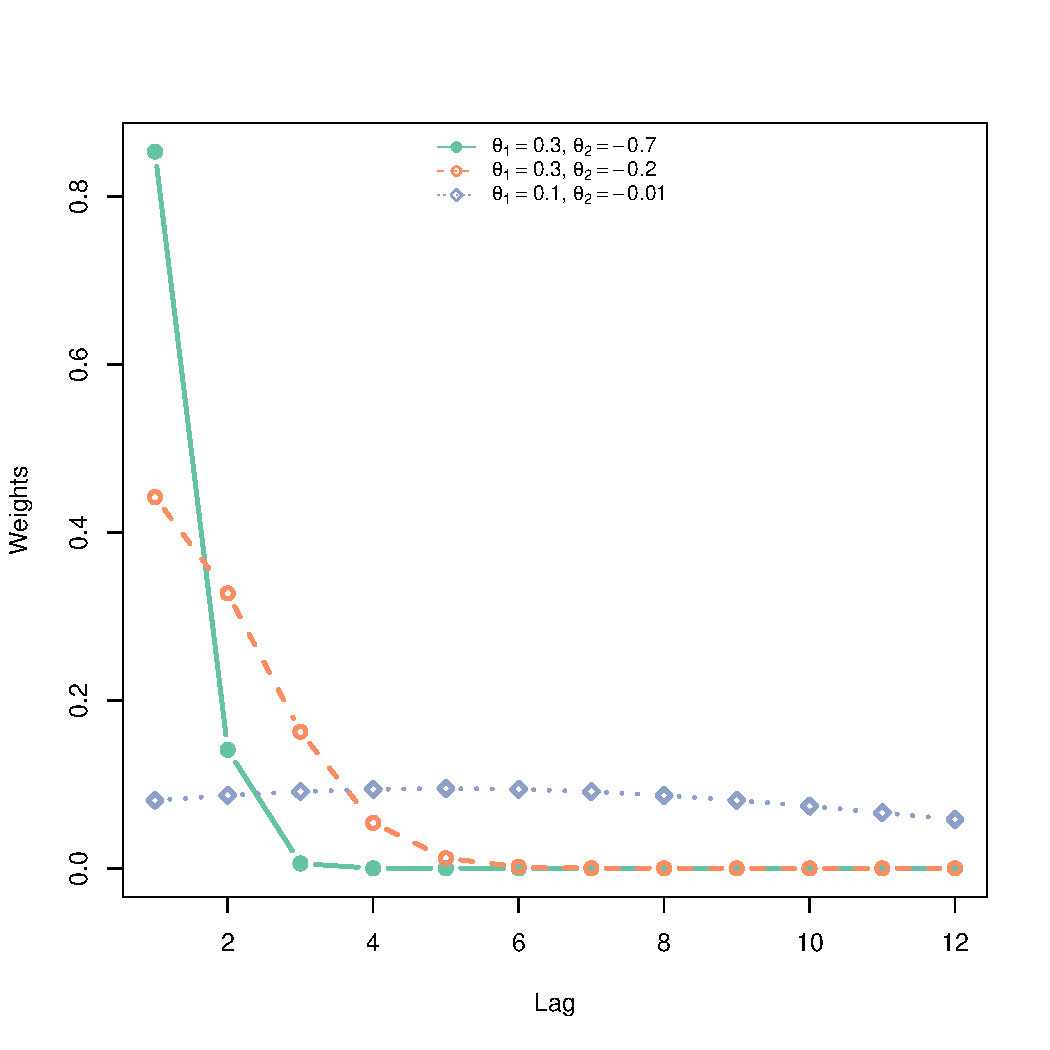
\includegraphics[width=0.5\linewidth]{../../figure/weight}
%\label{fig:weight}
%\end{figure}
%\begin{itemize}
%	\item Flexible and able to capture the evolution of lag effects smoothly. Recent lags have larger effects\\
%	\item Weighted sum is a non-linear combination of origin variables. MIDAS can be estimated by non-linear least square (NLS). 
%\end{itemize}

%\end{frame}


	
	
\begin{frame}{Factor Models}
A few factors summarize many variables. Principal components regression; dynamic factor model. (Banbura, 2013). 
	\begin{block}{}
$$X_t = \lambda (L) f_t + e_t$$
$$f_t = \Psi (L) f_{t-1} + \eta_t$$
	\end{block}
Solved in a state-space form.\\
High frequency $f_t$ is aggregated to low frequency $ \textcolor{blue}{\mathbf{f_t}}$.



	 \begin{block}{}
$$ y_{t} =  \beta_0 +  \beta_1  \textcolor{blue}{\mathbf{f_t}}  + \epsilon_t \,  .$$
	\end{block}

	
	
	
\end{frame}




\begin{frame}{Statistical Learning Approach}
Other ways to achieve sparse models or avoid parameter proliferation: variable/feature/model selection, model averaging, or model ensemble. 
	\begin{itemize}%[<+-| alert@+>]
		%\item 
		\item penalized regression: ridge, Lasso  (De Mol et al., 2008).
		\item bagging (Inoue \& Kilian, 2008).
		\item boosting (Bai \& Ng, 2007).
		\item Bayesian model averaging
		(Koop \& Potter, 2004; Wright, 2009).
	\end{itemize}	
	
\end{frame}





%%%%%%%%%%%%%%%%%%%%%%%%%%%%%%%%%%%%%%%%%%%%%%%%%%%%%%%%%%%%%%%%%%%%%

\section{Model:  BSTS-U-MIDAS}

\begin{frame}{BSTS-U-MIDAS Model}

	\begin{itemize}
		\item State-space component:
		\begin{itemize}%[<+-| alert@+>]
		%\item 
			\item Bayesian Structural Time Series (BSTS) model decomposes the target variable into several stochastic processes.
		
		\end{itemize}
		
		\item Regression component:
				\begin{itemize}%[<+-| alert@+>]
					\item U-MIDAS model tackles mixed-frequency data.
					\item Spike-and-slab regression is used for variable selection to handle the high dimensionality problem.
					\item BMA deals with model uncertainty and instability.
				\end{itemize}
		
	\end{itemize}
\end{frame}
%%%%%%%%%%%%%%
\begin{frame}{Local Linear Trend Model with Regression}

	\begin{block}{}
\begin{itemize}
%	\abovedisplayshortskip = 9pt plus 3pt minus 5pt
	
	\item {Observation equation(level + regression): $$y_t = \mu_t + \beta x_t + \epsilon_{t}, \quad \epsilon_{t} \sim N(0, \sigma_{\epsilon}^2)$$}	
	\item {State equation 1 (random walk + trend): $$\mu_t = \mu_{t-1} + b_{t-1} + w_{1t}, \quad w_{1t} \sim N(0, W_{1})$$}	
	\item {State equation 2 (random walk for trend): $$b_t = b_{t-1} + w_{2t}, \quad w_{2t} \sim N(0, W_{2})$$}
\end{itemize}
	\end{block}
	

\end{frame}
%%%%%%%%%%%%%%%%%%%


\begin{frame}{BSTS Model cont.}

		\begin{itemize}	
			\item Assumption: 
			\begin{itemize}
			\item	$\epsilon_t$, $w_{1t}$ and $w_{2t}$  are independent,
			\end{itemize}	
			\item States to estimate $\alpha$:
			\begin{itemize}
			\item $\mu_t, b_t$; Kalman filter.			
			 \end{itemize}	
				
			\item Parameters to estimate $\theta$:
				\begin{itemize}
				\item $\theta_1$: $W_{1}, W_{2}$ for state component;
				\item $\theta_2$: $\beta, \sigma_{\epsilon}^2$  for regression component; spike-and-slab regression.
			    \end{itemize}

		\end{itemize}
		








\end{frame}


%%%%%%%%%%%%%%%%%%%

%\begin{frame}{U-MIDAS:mixed frequency/ragged data}
%	\structure{Vertical allignment (Altissimo et
%		al. ,2010)}
%\begin{block}{}
%	\begin{center}
%		$\begin{bmatrix}
%	y_{2nd \, quarter}  &  & \,\,\,\quad ;& y_{1st \, quarter} & &; ...\\
%	x_{May} & x_{Apr} & x_{Mar}; &  x_{Feb} & x_{Jan} & x_{Dec} ;...
%%		\end{bmatrix}$
%		
%	Alignment:	$\begin{bmatrix}	
%		
%		y_{2nd \, quarter} & |  & x_{May} & x_{Apr} & x_{Mar} \\
%		y_{1st \, quarter} & |  & x_{Feb} & x_{Jan} & x_{Dec} \\
%		... & |  & ... & ... & ...	
%		\end{bmatrix}$\\
%	\end{center}
%\end{block}
%$y_{2nd \, quarter}$ is what we want to forecast. We have $x$ up to May. Easy implement, but when new observation arrives, the balanced dataset changes, the correlations  change, and the stability of model may change.

%\end{frame}


%%%%%%%%%%%%%%%%%%%

\begin{frame}{Spike-and-Slab Prior}
\begin{block}{}	
	$$\beta_i \sim (1-\gamma_i) N(0, c \varphi^2)+\gamma_i N(\tilde{\beta_i},\varphi^2)$$
\end{block}

\begin{minipage}{0.5\textwidth}
	\begin{figure}[H]
		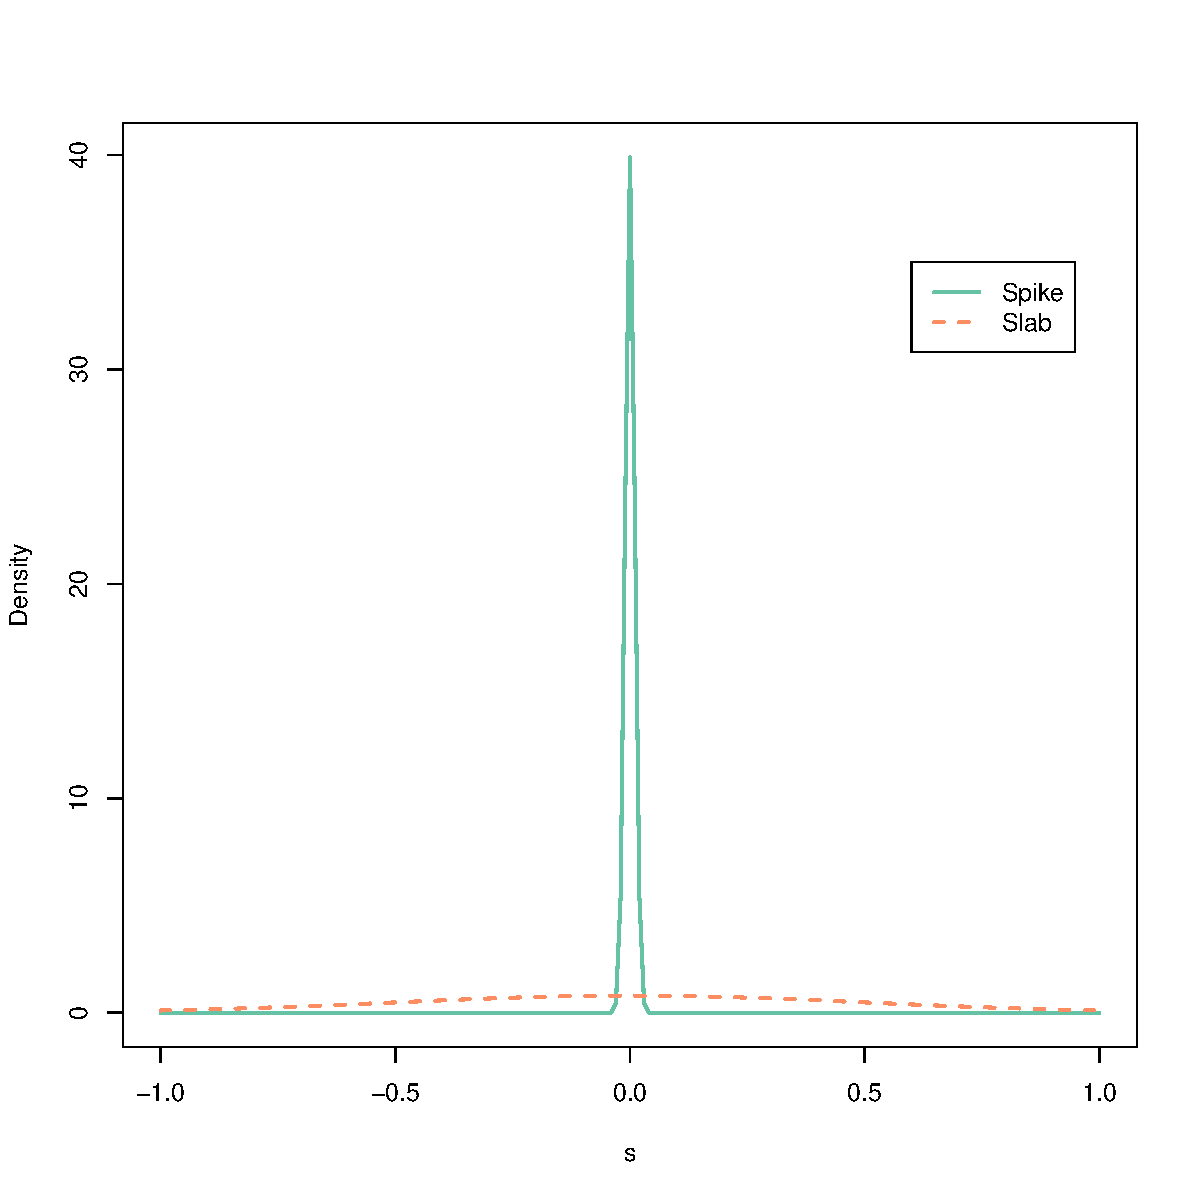
\includegraphics[width=0.8\linewidth]{../../thesis/draft/firstdraft/Figures/spike}
		%\caption{\label{fig:spike} }
	\end{figure}
\end{minipage} \hfill
\begin{minipage}{0.45\textwidth}
$\gamma_i = 0$: irrelevant predictor i has zero $\beta_i$. $c$ is very small number. A ``spike" at the origin.\\
 $\gamma_i = 1$: relevant predictor i has non-zero $\beta_i$. $\varphi^2$ is very large. Approximate to a ``slab".
\end{minipage}

	
$$\textcolor{blue}{\gamma_i} \sim  \pi_{i}^{\gamma_i}(1- \pi_{i})^{1-\gamma_i} \, .$$ 


 $\pi_i$ is predictor $x_i$'s probability of inclusion.

\end{frame}


%%%%%%%%%%%%%%%%%%


%%%%%%%%%%%%%%%%%%%

\begin{frame}{Estimation Using a Gibbs Sampler}
Alternates between draws of  $p(\alpha| \theta, \mathbf y_{1:t})$ and $p(\theta| \alpha,\mathbf y_{1:t})$.
\begin{enumerate}
\item  for state $\alpha$: $\mu, b$. 
 \begin{itemize}
 	\item    Draw from $p(\alpha | \mathbf{y_{1:t}}, \theta)$ using a stochastic versions of the Kalman smoother from Durbin and Koopman (2002);
 \end{itemize}
 
\item for parameters $\theta_1$ in state component :

 \begin{itemize}
 	\item   Draw for $W_1, W_2$ from independent inverse Gamma distributions given $\alpha, \mathbf{y_{1:t}}$. 
 \end{itemize}

\item for parameters $\theta_2$ in regression component. 
  \begin{itemize}
  	\item  Draw from $p(\beta, \sigma^{-2},\gamma) = p(\beta \mid \gamma, \sigma^{-2})p(\sigma^{-2} \mid \gamma )p(\gamma)$ using spike-and-slab prior with  “stochastic search variable selection”(SSVS) algorithm given $\alpha, \mathbf{y_{1:t}}$. 
  \end{itemize}

\end{enumerate}


\end{frame}




%%%%%%%%%%%%%%%%%%

%%%%%%%%%%%%%%%%%%%

\begin{frame}{Bayesian Model Averaging}
With a sequence of posterior \{$\alpha_1, \theta_1; \alpha_2, \theta_2,...$\} from MCMC, 
\begin{itemize}
\item Get predictive distribution for one step ahead forecast for target variable
$p(\tilde{y}_{t+1} | \mathbf{y_{1:t}, \mathbf{x_{1:(t+1)}}})$.

\item By averaging over draws for $\tilde{y}_{t+1}$, get a point forecast, which is a form of Bayesian model averaging and accounts for the model uncertainty. \\

\item Average over draws for $\gamma_i$ to get predictor $x_i$'s probability of inclusion  $\pi_i$. 
\end{itemize}
\end{frame}




%%%%%%%%%%%%%%%%%%



%%%%%%%%%%%%%%%%%%%%%%%%%%%%%%%%%%%%%%%%%%%%%%%%%%%%%%%%%%%%%%%%%%%
\section{Empirical Application}


%%%%%%%%%%%%%%%%%%%

\begin{frame}{Empirical Application: Data}



\begin{itemize}
	
	\item Quarterly GDP.
	 \begin{itemize}
		\item Seasonally adjusted. 
	    \item Log differenced for comparison with ARIMA. 
	\end{itemize}
	\item Daily(include $22 \times 12-1$ lags): 
	\begin{itemize}
		\item Toronto Stock Exchange (TSX) index, 
		\item daily West Texas crude oil prices,
	\end{itemize} 
	\item Monthly(include $3\times8 -1$ lags):
	
	\begin{itemize}
		\item unemployment rate, 
		\item monthly spread between interest rates of 10 year government bonds and 3 month treasure bill,
		\item monthly housing starts.
		
	\end{itemize} 
\end{itemize}
Detrend ,deseasonalize, and standardize the predictors.\\
Total $600$ predictors; $114$ observations.
	
\end{frame}


\begin{frame}{One Step Ahead Forecast of GDP Growth}
MCMC: 10,000 iterations and discarded the first 2,000 as burn in. 
\\The default priors in R package ``bsts" (Scott, 2015), except choosing the ``expected model size" to 4.  
\begin{figure}
\centering
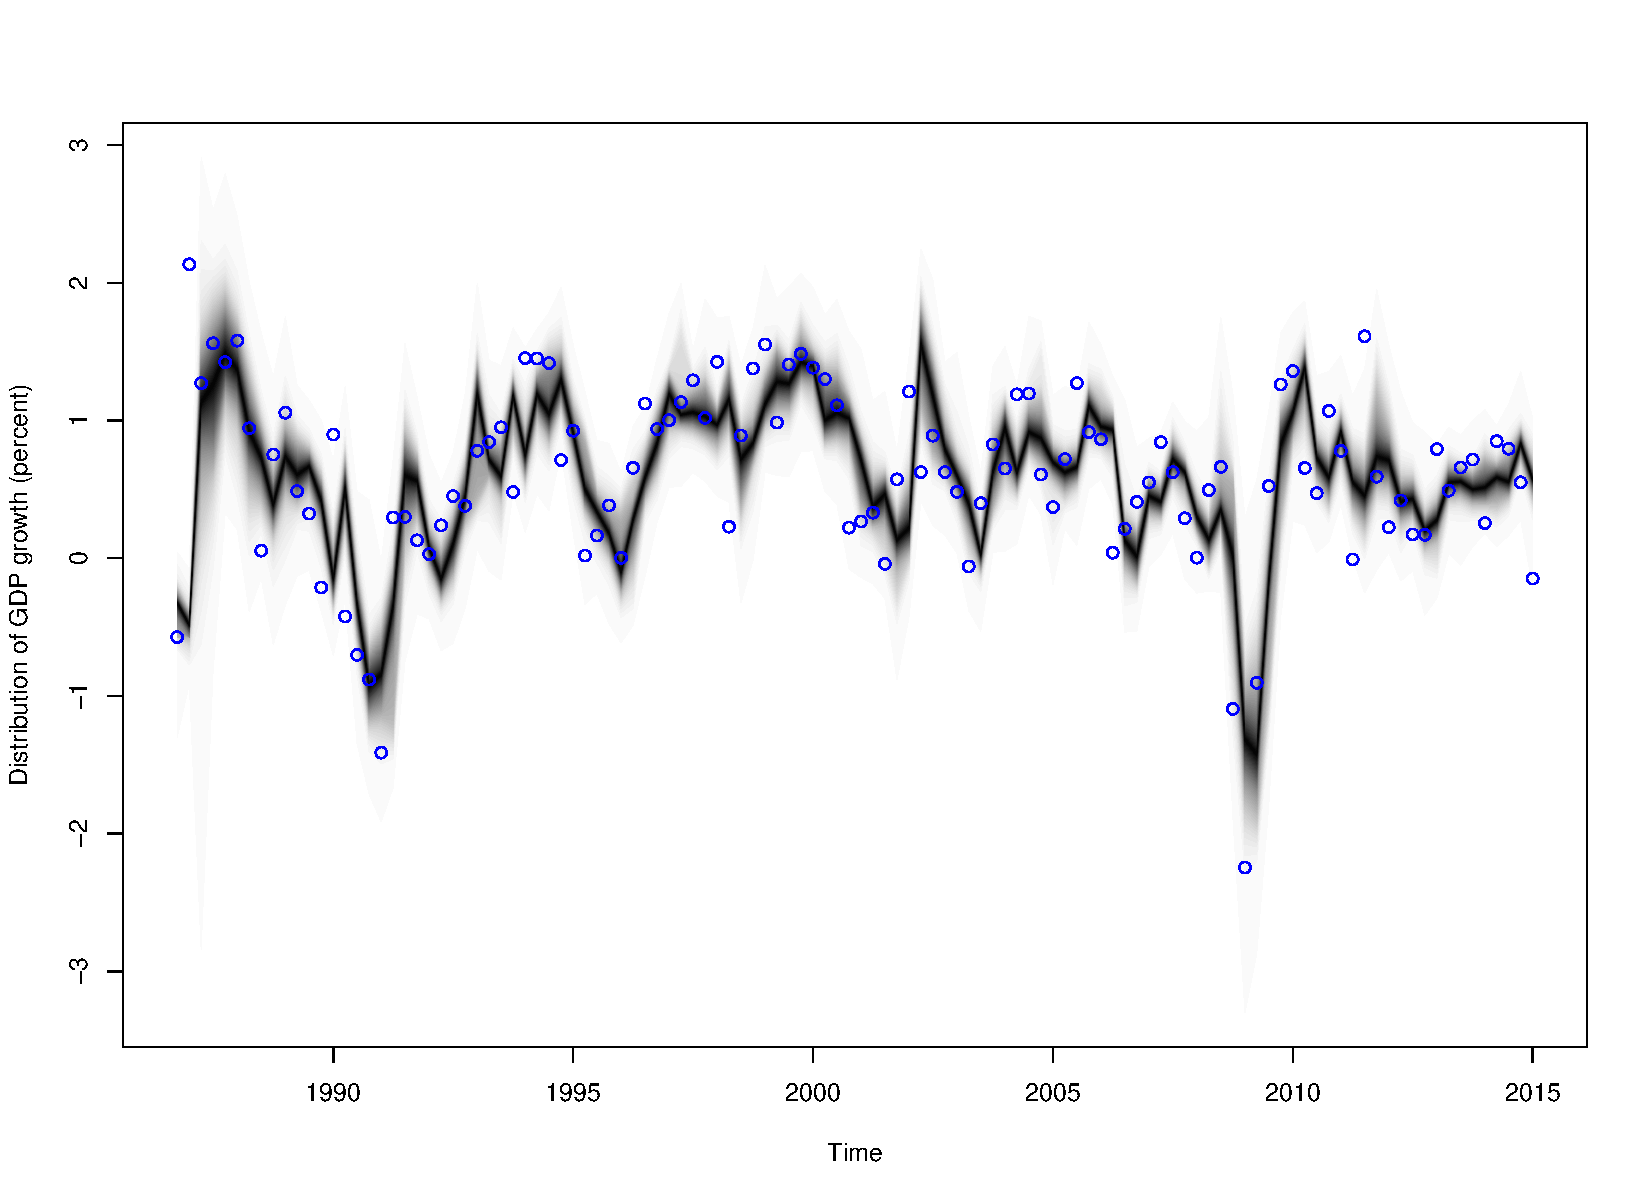
\includegraphics[width=0.6\linewidth]{../../thesis/draft/firstdraft/Figures/forecast_distribution}
%\caption{One s}
\label{fig:forecast_distribution}
\end{figure}

\end{frame}







\begin{frame}{Contributions of States for GDP Growth}
Add an AR(4) term in the state equation. The AR term is relatively stable, and the trend component is more volatile. The regression component exhibits the most variation, which  helps to capture the turning points  of the GDP growth. 
\begin{figure}
\centering
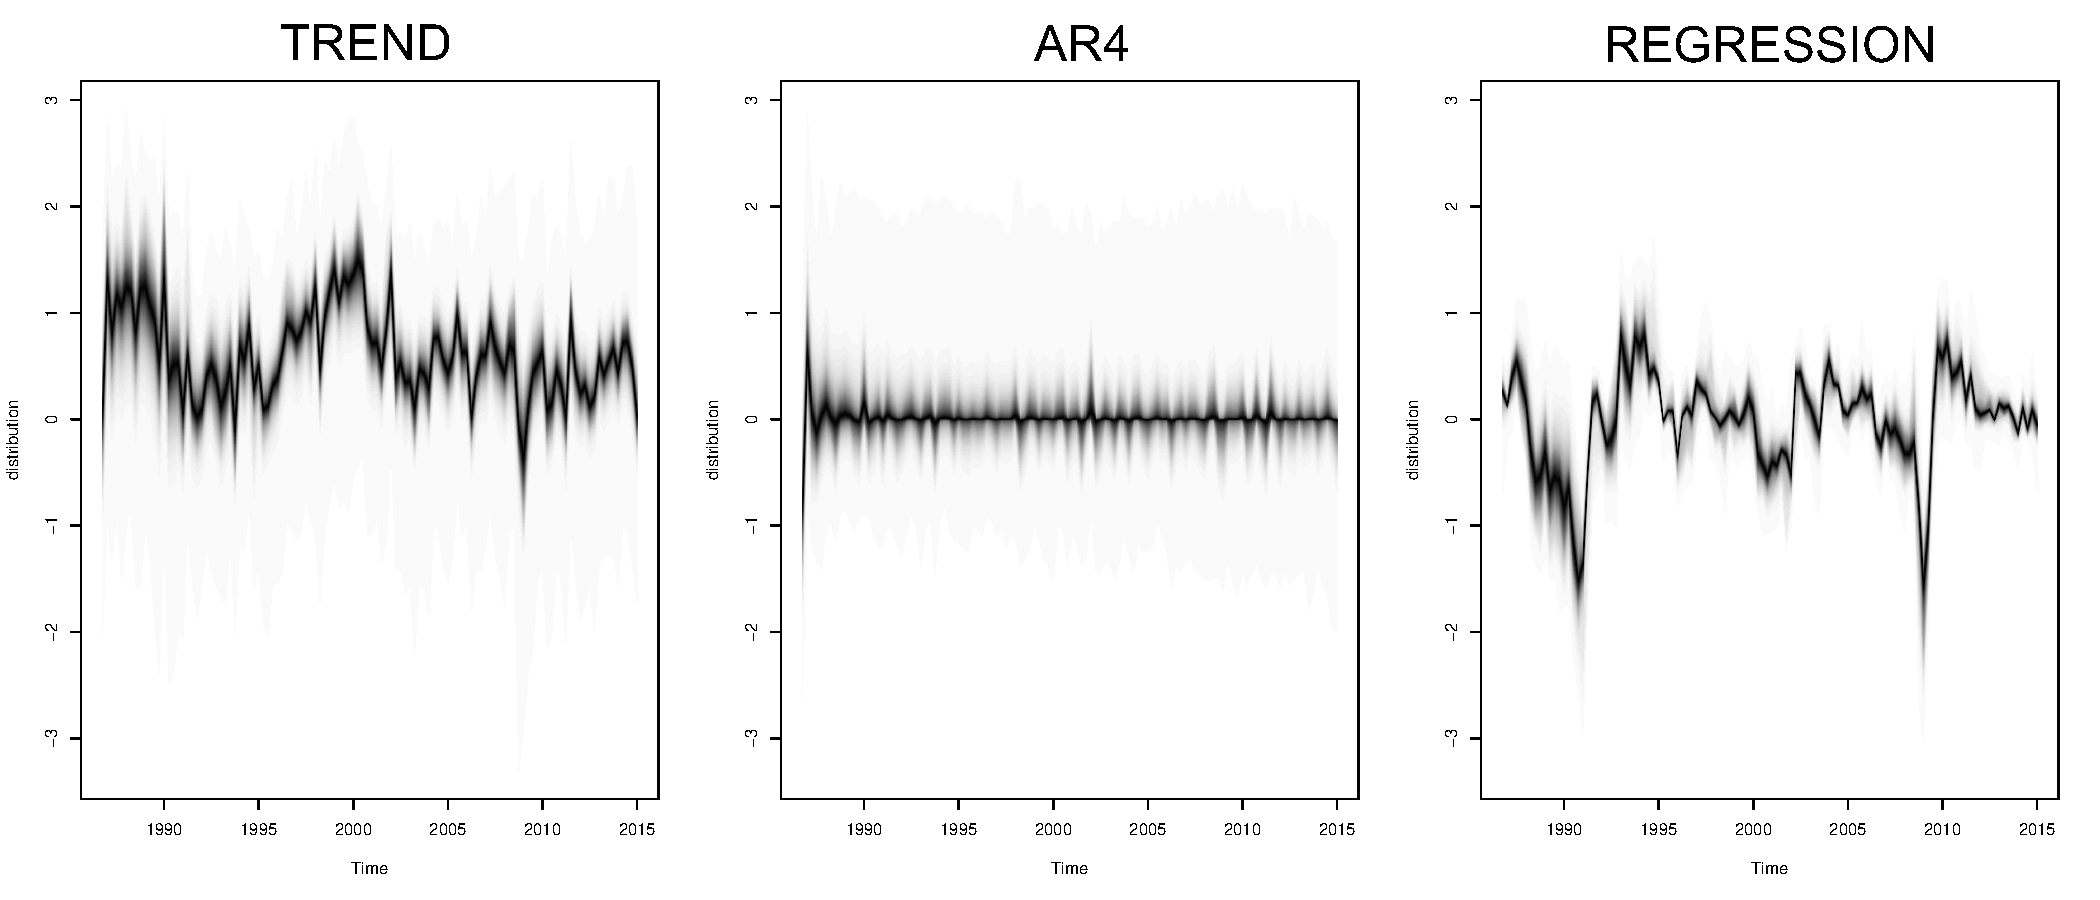
\includegraphics[width=0.9\linewidth]{../../thesis/draft/firstdraft/Figures/components}
%\caption{}
\label{fig:components}
\end{figure}
\end{frame}
	
\begin{frame}{The Cumulative Absolute One Step Ahead Forecast Error}
During 2008 to 2009 financial crisis, the cumulative error for model without regression component increases rapidly, however the error for BSTS with regression increases at a constant rate, which shows its robustness. 
	\begin{figure}
		\centering
		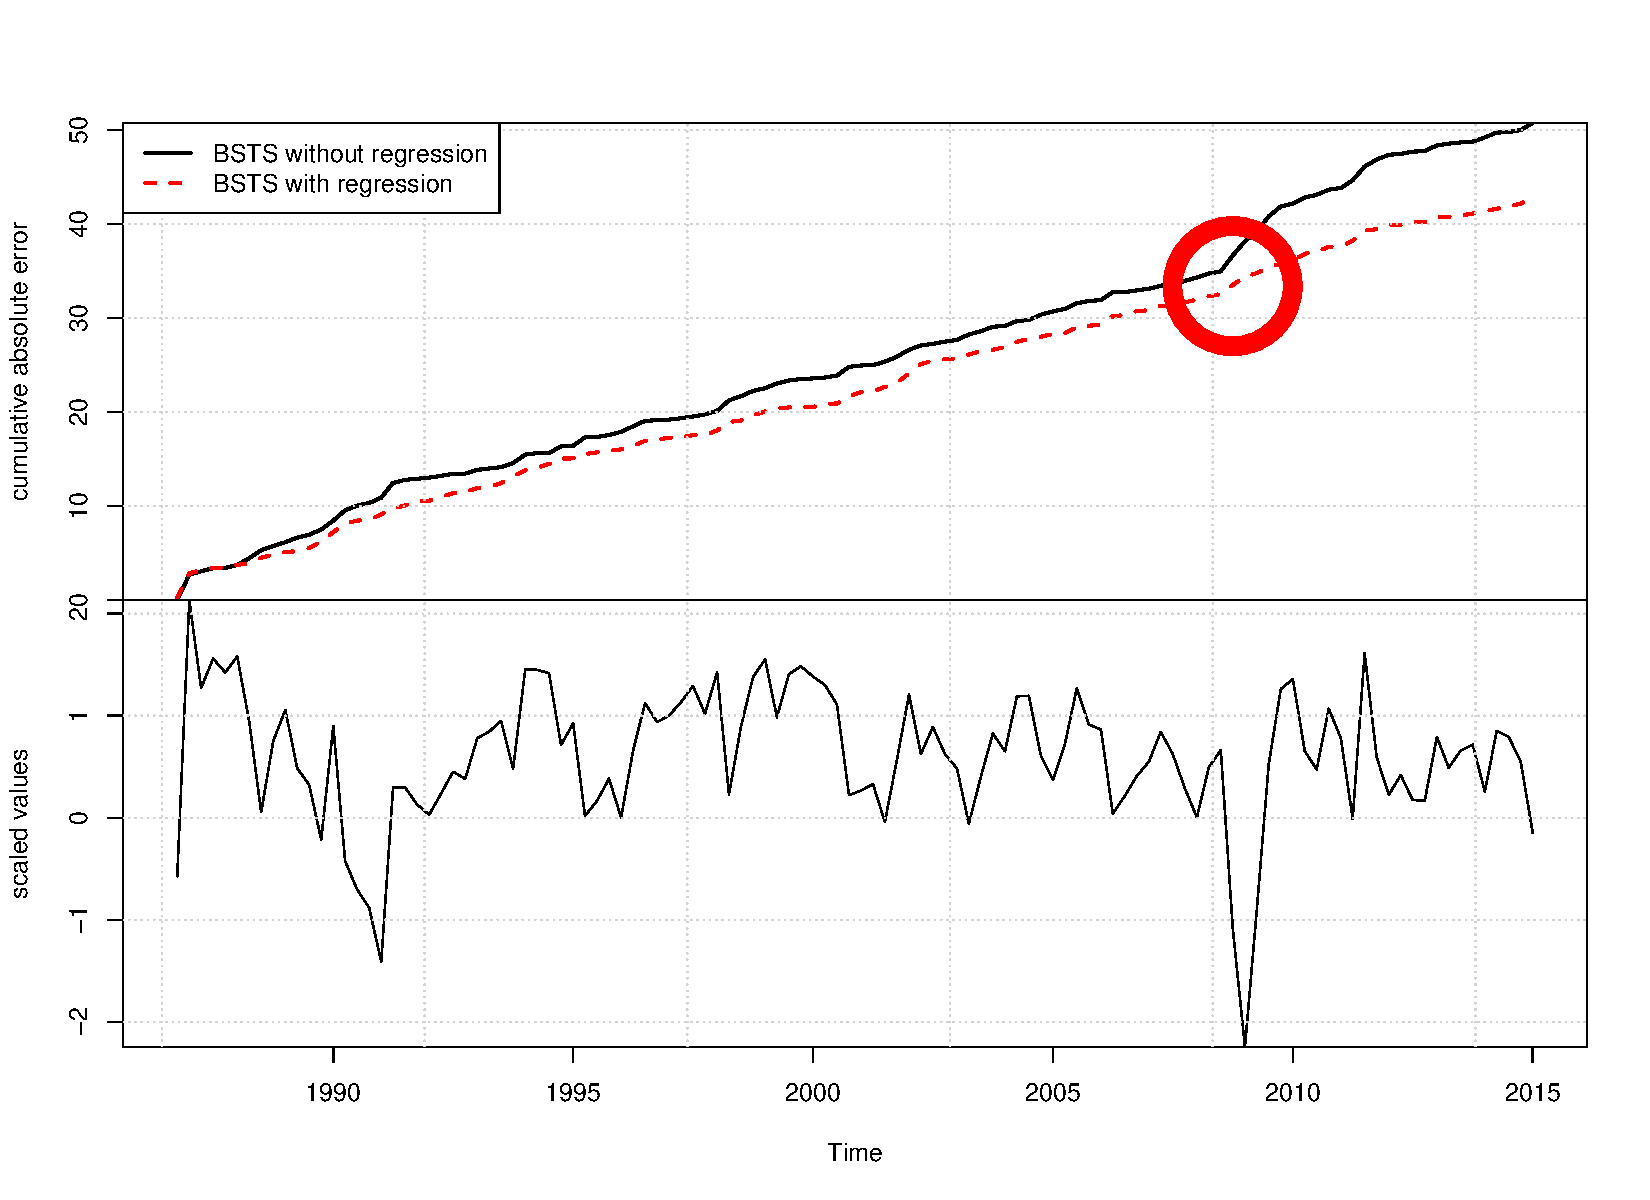
\includegraphics[width=0.5\linewidth]{../../thesis/draft/firstdraft/Figures/cumulative_errors}
		%\caption{}
		\label{fig:cumulative_errors}
	\end{figure}
 	
	
\end{frame}
	
	
\begin{frame}{Predictors with High Inclusion Probability}
The inclusion probability of predictor indicates its ability of helping prediction. A white bar indicates positive relationship,  black indicates  negative. 

\begin{minipage}{0.5\textwidth}
	\begin{figure}[H]
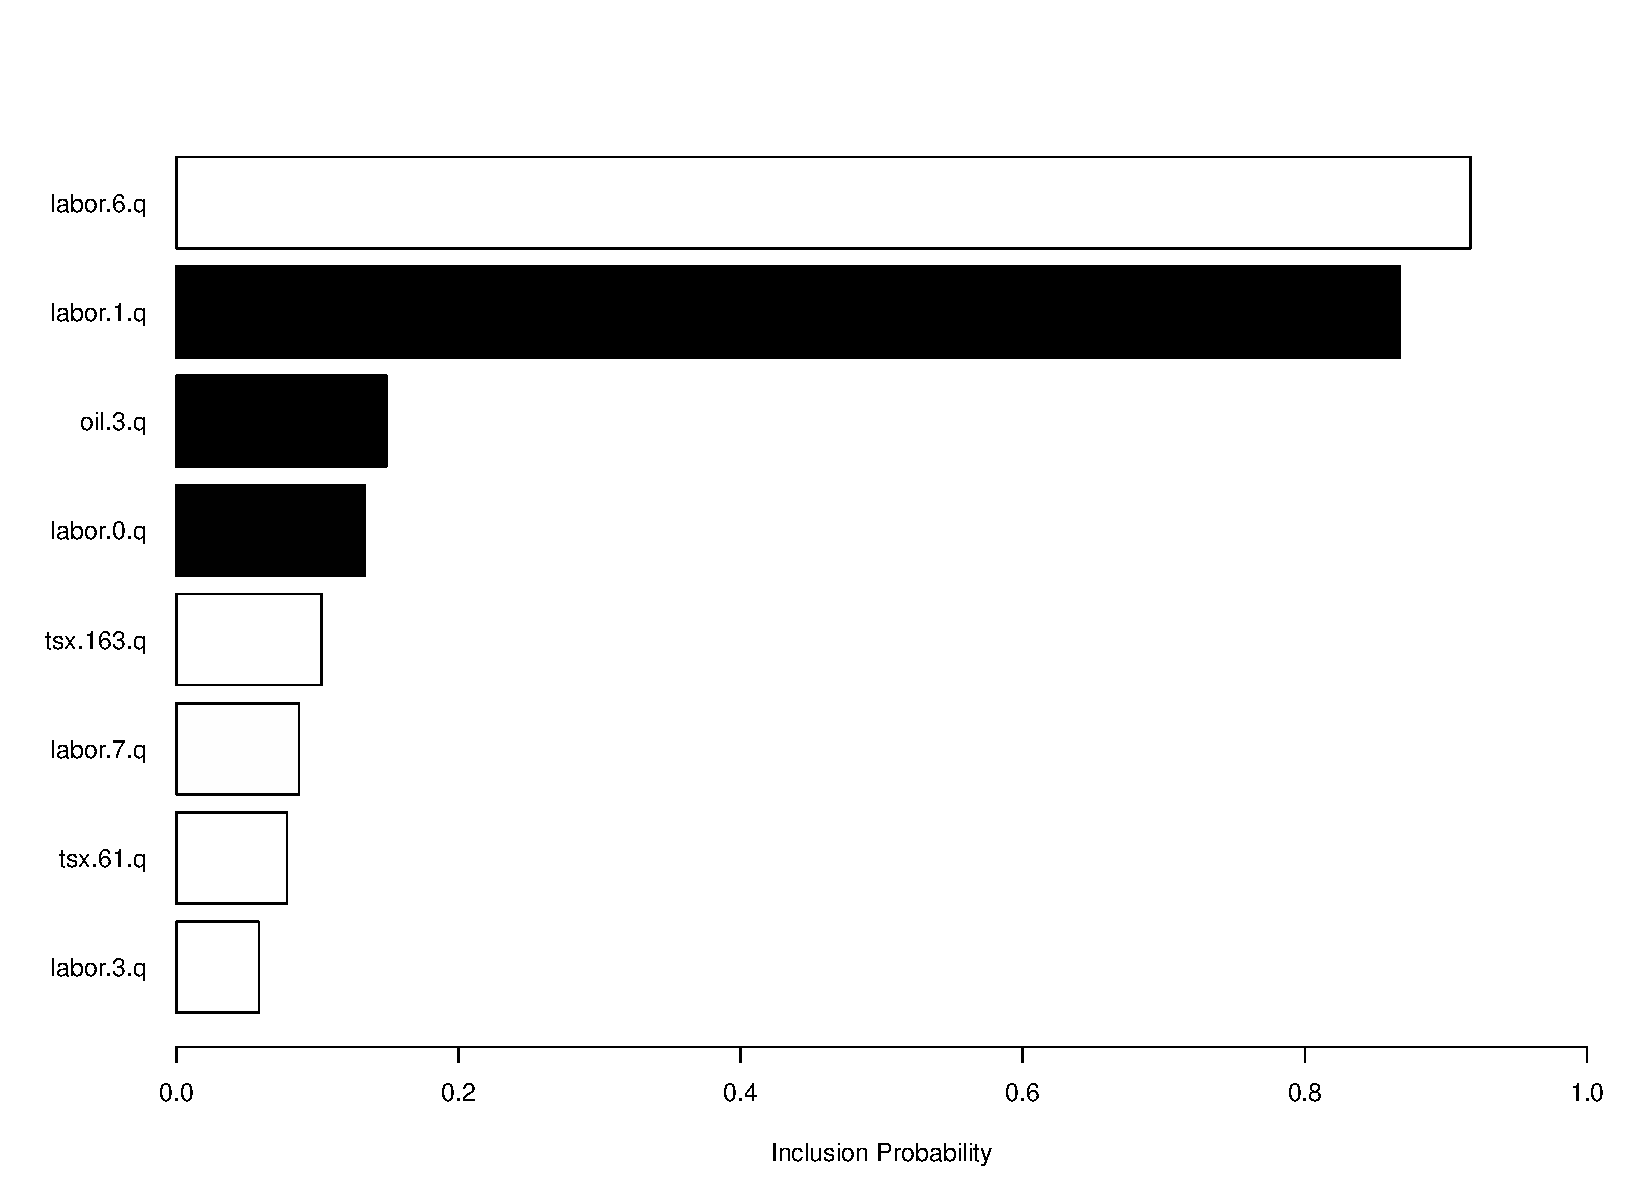
\includegraphics[width=1\linewidth]{../../thesis/draft/firstdraft/Figures/Coefficients}
		%\caption{\label{fig:spike} }
	\end{figure}
\end{minipage} \hfill
\begin{minipage}{0.46\textwidth}
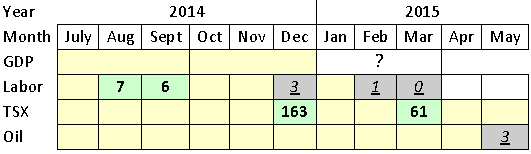
\includegraphics[width=1\linewidth]{../../thesis/draft/firstdraft/Figures/MonthQuarterYear}
\end{minipage}
It shows most of models are sparse. A combination of high frequency data works as a good predictor, which is similar to MIDAS weighting scheme and factor. 	
\end{frame}




\begin{frame}{Comparison with ARIMA, and Boosting}
Choose 2003 to 2015 as test period. ARIMA is benchmark; Boosting model is flexible; nonlinear . 
\begin{figure}
\centering
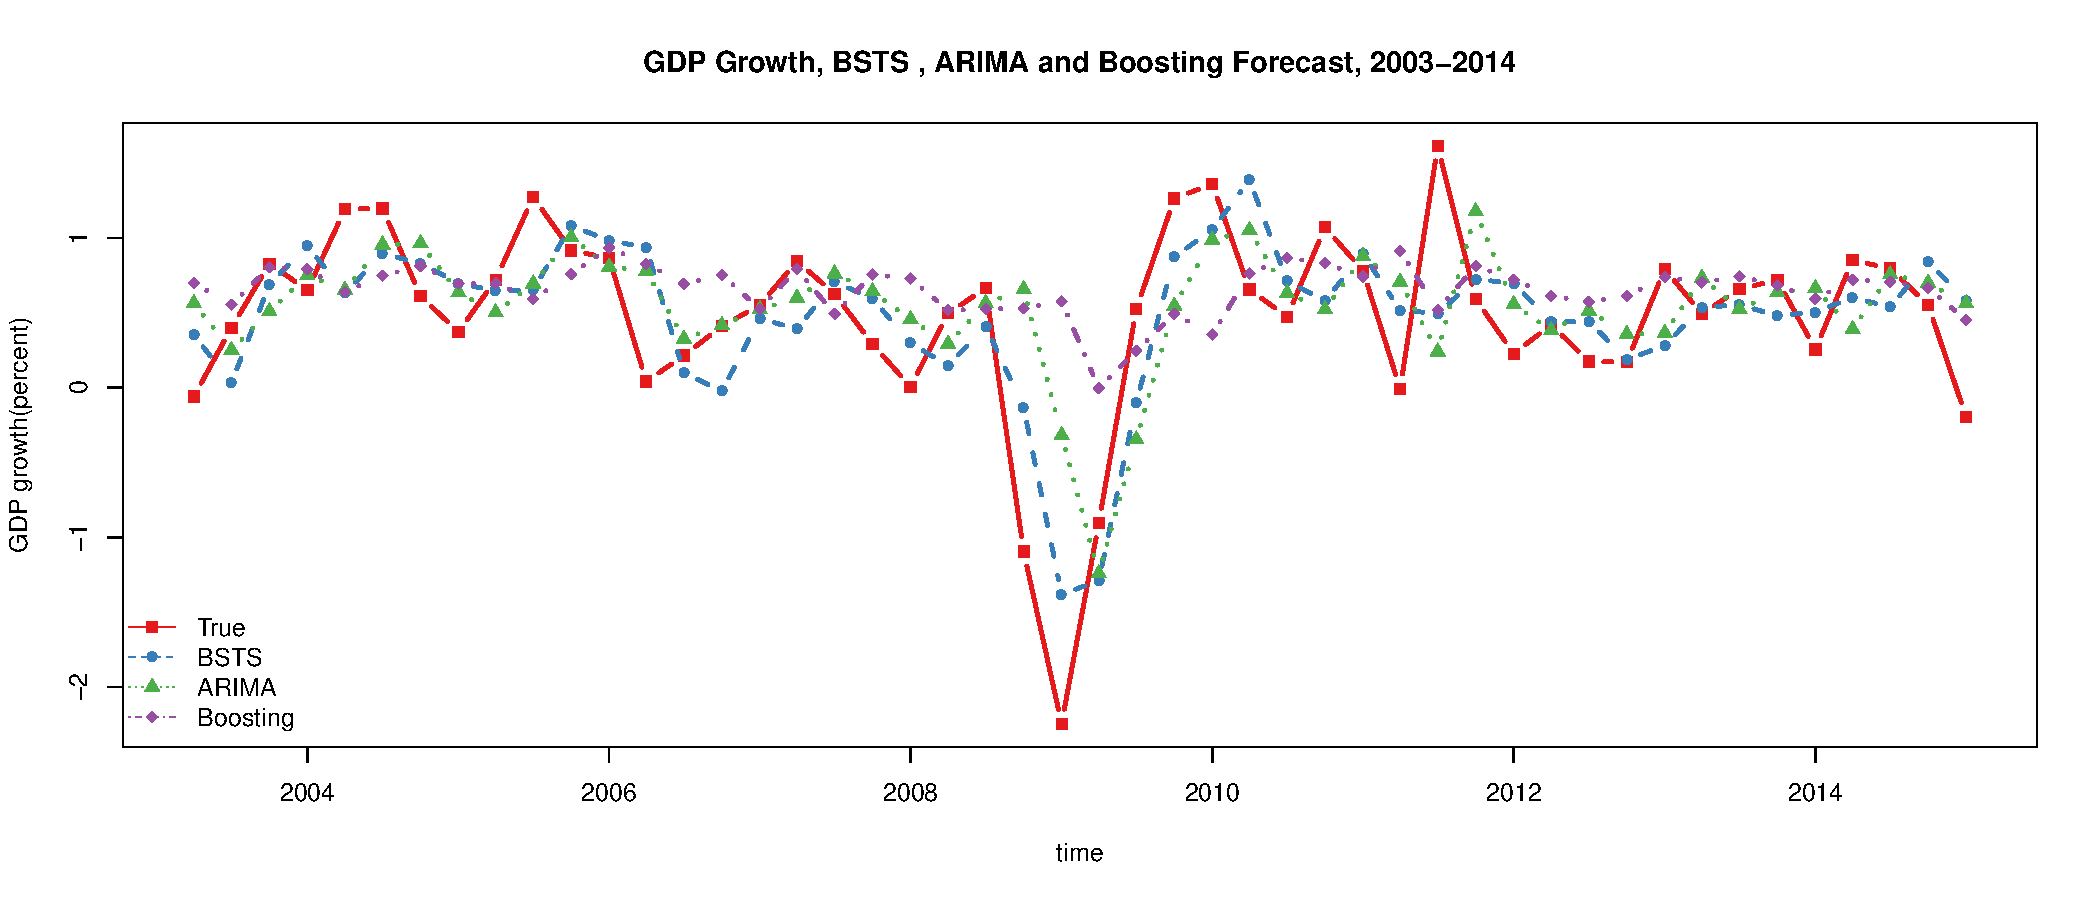
\includegraphics[width=0.9\linewidth]{../../thesis/draft/firstdraft/Figures/bsts_arima_boost}
%\caption{}
\label{fig:bsts_arima_boost}
\end{figure}
BSTS outperforms other two due to better performance (MAPE) during 2008 to 2009 financial crisis. 

	
\end{frame}


\begin{frame}{Comparison in GDP Level}
\begin{figure}
\centering
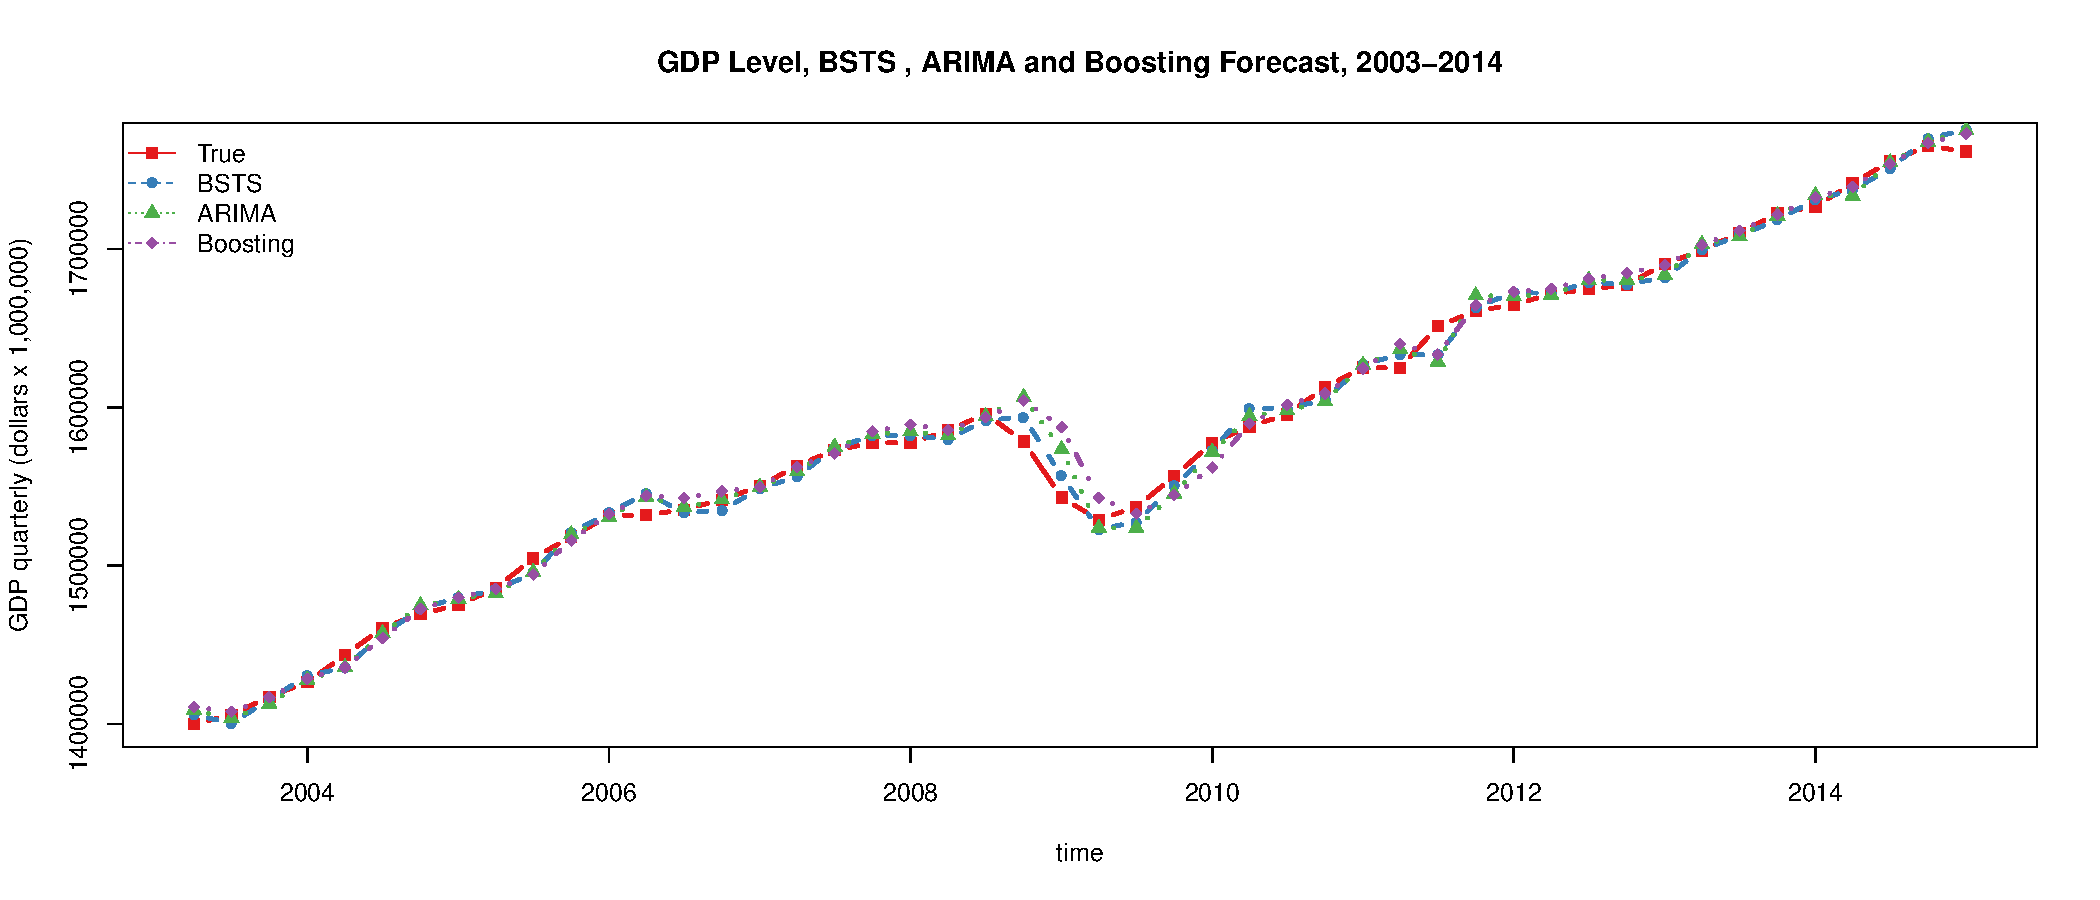
\includegraphics[width=1\linewidth]{../../thesis/draft/firstdraft/Figures/bsts_arima_boost_gdp}
%\caption{}
\label{fig:bsts_arima_boost_gdp}
\end{figure}
% Please add the following required packages to your document preamble:
% \usepackage{booktabs}
\begin{table}[h]
	\centering
	\begin{tabular}{@{}llll@{}}
		\toprule
		& BSTS   & ARIMA    & Boosting   \\ 
		\midrule
		MAPE     & 0.356 &0.401 & 0.405  \\
		\bottomrule
	\end{tabular}
	%\caption{Comparison of forecast error 2003-2015}
	%\label{ErrorCom}
\end{table}
\end{frame}


%%%%%%%%%%%%%%%%%%%%%%%%%%%%%%%%%%%%%%%%%%%%%%%%%%%%%%%%%%%%%


\section{Conclusions}



\begin{frame}{Conclusions}
	
Advantage of BSTS-U-MIDAS:
\begin{itemize}
	\item flexible for handling high frequency and ragged
	data,
	\item capable of capturing the structural breaks or	turning points,
	\item robust to irrelevant or redundant	variables,
	\item easy to incorporate new information of predictors to update the forecast.
\end{itemize}
Further study:
\begin{itemize}
	\item test the model based on simulated data,
	\item use historical data to improve the prior,
	\item model volatility of economic variable instead of the level or return. 

\end{itemize}
\end{frame}




\end{document}
